Where we previously assumed the existence of an ideal payment procedure, we now
describe the technical construction for the moneTor payment scheme. The protocol
setup and algorithmic overview of the payment layer is covered in this chapter.

\subsection{Payment Protocols}

In this section we specify formal protocols that comprise the payment
scheme. All protocols are either two or three party interactions between a
subset of the following roles: $C$ (client), $R$ (relay), $E$ (end user: either
a client or relay), $I$ (intermediary), and $L$ (ledger). At this level, we
assume that one client is paying one relay through a single channel and that
communication lines will be appropriately anonymized by the Tor networking
protocol.

\textbf{Bolt} The moneTor payment scheme is a superset of Bolt's three-party
bidirectional micropayment channels. As such, we adopt its nomenclature where
possible but adapt it to our concepts of ledgers, clients, and relays. The
following is brief outline of the prerequisite micropayment channel procedures
defined in Bolt. We refer the reader to the original paper for more detailed
specifications~\cite{green2017bolt}.

\begin{itemize}
\item \textbf{KeyGen}: Any party generates a cryptographic keypair
\item \textbf{Init-E}: $E$ initializes half of a micropayment channel by
  escrowing funds on $L$
\item \textbf{Init-I}: $I$ initializes half of a micropayment channel by
  escrowing funds on $L$
\item \textbf{Establish}: $E$ and $I$ interact to establish a new micropayment
  channel from their respective halves
\item \textbf{Pay}: $C$ interacts with $I$ and $R$ to send a single micropayment to $R$
\item \textbf{Refund}: $E$ closes a channel on $L$ and makes a claim on
  the escrow.
\item \textbf{Refute}: $I$ closes a channel on $L$ and makes a claim on
  the escrowed.
\item \textbf{Resolve}: $L$ determines the final balance of funds awared to
  each party.
\end{itemize}

While anonymous micropayment channels present a tremendous advance for many
applications, the relatively heavy cryptography ($37-100\ ms$) and communication
(7 message legs) is a prohibitive expense for Tor relay payments.\footnote{In addition to
concerns regarding global network overhead, it is also desirable to keep the
barrier of entry low for smaller relay operators.} To overcome this
barrier, we present a new payment layer design enabling far more efficient
nanopayments that will satisfy our constraints.

\textbf{moneTor} The moneTor construction makes use of the existing anonoymous
micropayment structure to facilitate \emph{locally transparent nanopayments}. In
this scheme, \emph{nanopayment channels} are established in place of a single
micropayment operation. These lightweight channels allow the client to send $n$
number of unidirectional nanopayments to the relay. Each payment represents a
fixed value $\delta$, established at the start of the channel. The payments
themselves are \emph{locally transparent} in the sense that each nanopayment in
the same channel is trivially linked to each other. However, the nanopayment
channels themselves are unlinkable to other nanopayment channels and
micropayment operations.

\begin{figure}[h] \centering
  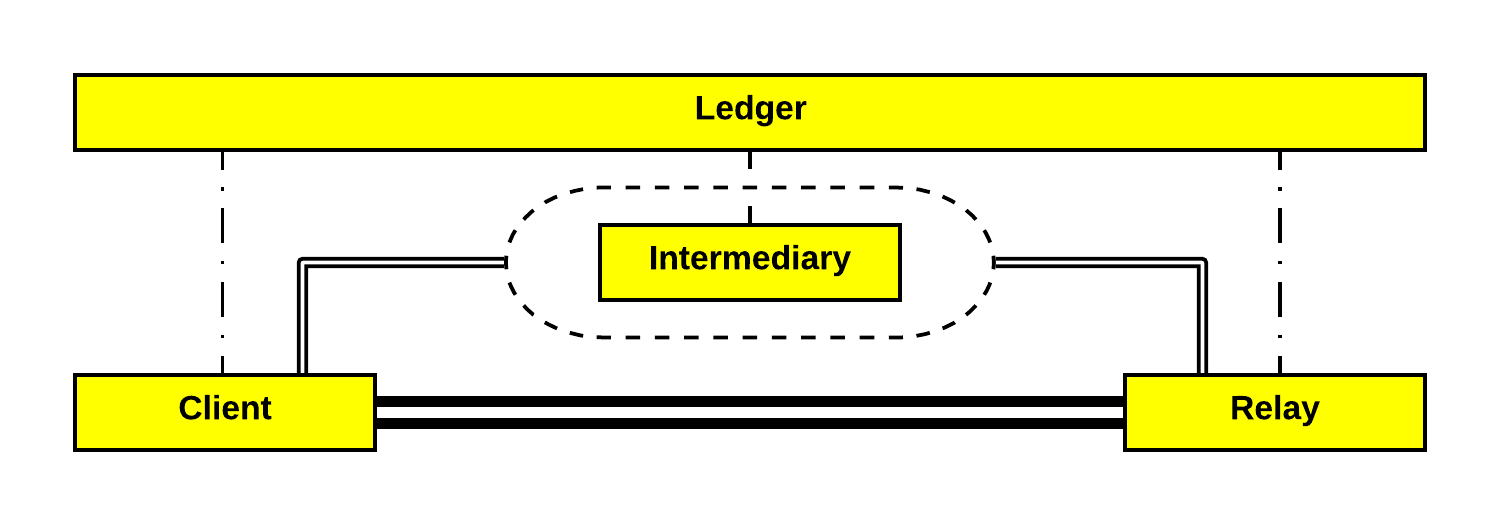
\includegraphics[scale=0.6]{images/party_diagram.png}
  \caption[Payment Roles]{Payment Roles --- Dashed lines represent periodic
    transactions, thin double lines indicate micropayment channels, and thick
    double lines indicate a nanopayment channel. The gray area around the
    intermediary represents a notion of payment anonymity for the end users.}
  \label{fig:parties}
\end{figure}

Generic parties $C$ and $R$ can construct a nanopayment channel once both have
completed $Establish$ with a common intermediary $I$. We define the following
set of protocols needed to manage nanopayments.

\begin{itemize}
\item \textbf{Nano-Setup} $C$ and $I$ interact to prepare a nanopayment channel on top
  of their existing micropayment channel.
\item \textbf{Nano-Establish} $C$ sends her nanopayment channel information to $R$,
  who establishes it with $I$ on top of their existing micropayment channel.
\item \textbf{Nano-Pay} $C$ sends a single nanopayment channel to $R$. This is
  repeatable for up to $n$ operations.
\item \textbf{Nano-Close-R} $R$ closes his nanopayment channel with $I$.
\item \textbf{Nano-Close-C} $C$ closes her nanopayment channel with $I$. Note that
  this must happen after \emph{Nano-Close-R}.
\end{itemize}

We also specify the following modified channel conflict resolution procedures to
ensure secure closure properties for the nanopayment scheme.

\begin{itemize}
\item \textbf{Nano-Refund} $E$ closes channel on $L$.
\item \textbf{Nano-Refute} $I$ closes channel on $L$.
\item \textbf{Nano-Resolve} $L$ makes final determination on both micropayment and
  outstanding nanopayment balances.
\end{itemize}

The core of our nanopayment scheme is inspired by the classic \emph{Payword}
two-party micropayment scheme in which payments are encoded by successively
revealed preimages in a precomputed hash chain~\cite{rivest1996payword}. Hash
chains are perhaps the most efficient known method for representing payments. In
contrast to the expensive zero-knowledge proofs and signatures involved in
anonymous micropayments, hash chain payments can be computed one the order of
millions of hashes per second and conferred with a single 256 bit message, or
one Tor cell.

The challenge in this construction is to securely integrate the hash chain
concept into an existing three-party anonymous micropayment channel setup such
that all parties maintain secure cryptographic ownership of their funds at all
steps. At the same time, we must ensure that no deanonymizing information is
leaked outside of the nanopayment channel context. We proceed to present a
concrete scheme which incurs an overhead penalty of approximately two
micropayment operations per nanopayment channel, one at the beginning and one at
the end of the channel life cycle.

\subsection{Nanopayment Protocols}
In this section, we provide a summarized intuition for the basic steps in the
payment protocol. A more formal algorithmic treatment of the steps are provided
in Appendix~\ref{chap:algorithms}.

\textbf{Nano-Setup} At the start of this protocol, $C$ has access to a
micropayment wallet $w$ that enables her to operate her micropayment channel
with $I$ as well as a refund token $rt$ that entitles her to claim her current
funds on $L$ should $I$ misbehave or go offline. To construct a nanopayment
channel, $C$ first generates an array of values $hc$ of length $n$ where
$hc_i = H(hc_{i+1})$ and $hc_n$ is a random number. The root of the hash chain
$hc_0$ is used to create a globally unique nanopayment token $nT$ that encodes
the public parameters of the channel including the length $n$ and the
per-payment value $\delta$. $C$ sends $I$ a commitment to a fresh nanopayment
channel parameterized by $nT$ along with a zero-knowledge proof of the following
statements:

\begin{enumerate}
\item The nanopayment wallet $nw$ is well-formed from $w$
\item $C$ has ownership of a micropayment channel containing at least $n *
  \delta$ funds.
\end{enumerate}

$I$ verifies these messages and blindly supplies $C$ with a new refund token
$nrt$ that entitles $C$ to cash out the full balance of the micropayment channel
along with any nanopayments to $L$. $C$, now protected against misbehavior by
$I$, agrees to send a revocation token $\sigma_w$, which revokes her right to
use $w$ or $rt$. $I$, now protected against double spending by $C$, can safely
inform $C$ that the nanopayment channel has been set up successfully.

\textbf{Nano-Establish} At this point, $C$ sends $R$ the same $nT$ token used to
setup the channel with $I$. $R$ uses the token to initiate her end of the
nanopayment channel with $I$ by executing essentially the same procedure that
$C$ used in \emph{Nano-Setup}. The nanopayment channel is now fully established and
ready to be used. A key observation is that both ends of the channel ($C$-$I$
and $R$-$I$) are rooted at the same hash chain root $hc_0$.

\textbf{Nano-Pay} To make the next $i^{th}$ payment, $C$ simply sends the next
hash preimage $hc_i$ to $R$. Knowledge of this preimage $hc_i$ is sufficient for
$R$ to prove possession of a nanopayment. At any given time, $R$ can broadcast
the tuple ($nrt$, $hc_i$) to $L$ to prove ownership of the correct balance of
funds. Notice that this action simultaneously reveals $hc_i$ to $I$, who can
then claim an equivalent value of funds from $C$. As a result, the
scheme satisfies a correct-by-construction property of \emph{atomicity}
whereby both legs of the protocol are finalized at the same time.

\textbf{Nano-Close} After some number of payments $k < n$ has transpired, $C$ and $R$ will both wish
to close their nanopayment channels through $I$. In this process, the $R$-$I$ leg
must be closed before the $C$-$I$ leg. This is due to the unidirectional nature
of nanopayment channels. Since payments are flowing form $C$ to $R$, $I$ must
first determine its debt to $R$ in order to know how much it can claim from $C$.

$R$ first sends to $I$ a commitment to a new micropayment wallet $w'$ and a
zero-knowledge proof of the following statements:

\begin{enumerate}
\item $w'$ is well-formed from $w$
\item The balance of $w'$ is equal to the sum of the previous wallet $w$ and
  $\delta * k$
\end{enumerate}

Once verified, $I$ issues a refund token $rt'$ on the new funds. $R$ agrees to
invalidate the nanopayment channel by issuing a revocation token $\sigma_{nw}$
to $I$. $I$ and $R$ proceed to create a blind signature on $w'$ thus validating
the wallet for future use.

Once $I$ has closed his nanopayment channel leg with $R$, $I$ and $C$ are free
to complete the exact same close protocol. All parties are now reverted to the
original state they occupied prior to \emph{Nano-Setup} save for a securely updated
balance.

\textbf{Nano-Refund, Nano-Refute, Nano-Close} Honest parties will not typically
close active nanopayment channels on the ledger, opting instead to run Bolt
micropayment closure procedures when they wish to cash out. However, in the
event of malicious behavior or premature abortion, \emph{Nano-Refund} and
\emph{Nano-Refute} outlines procedures for $E$ and $I$ to withdraw funds on the
ledger at any given step with the latest payment information. After a set amount
of time allowing for the counterparty to reciprocate, the ledger runs
\emph{Nano-Close} to make a final publically verifiable determination on the
final balance.

\subsection{Payment Security and Anonymity}
Our security model must account for both privacy and payment security. The
privacy threat model is derived from the local active adversary paradigm
ubiquitously found in Tor research~\cite{dingledine2004tor}. 

Our threat model for payment security is similar to those found in prior works
in blockchain micropayment channels~\cite{poon2016bitcoin}. In such models, the
user is protected from malicious intermediaries by the ability to prove
misbehavior to a global ledger. The security of the ledger will be subject to
the guarantees made by the cryptocurrency interface~\cite{back2014enabling,
  poon2017plasma}. This is in direct contrast to prior Chaumian e-cash proposals
that employ the \emph{honest but curious} model for the central bank. Indeed,
this is the basis for the difference in terminology between prior \emph{central
  banks} and the moneTor \emph{ledger}.

Informally, we claim the following anonymity guarantees relative to unmodified Tor:

\begin{enumerate}
\item Additional parties needed to operate the moneTor system (i.e. ledgers and
  intermediaries) cannot extract any more information about a given client than
  what would be known by adding a second middle relay to the circuit.
\item Excluding side channels, circuits do not leak any more information other than the single bit needed to differentiate premium and nonpremium users.
\end{enumerate}

Observing the cash-out transactions on the ledger does not reveal any information regarding the source of the payment. Moreover, any communication in our tripartite nanopayment protocol are protected by Tor circuits. Hence, relationship between Client to Intermediary, Client to Ledger, Relay to Intermediary and Relay to Ledger are themselves anonymized by Tor circuits. If some party abort, which induce a dispute on the Ledger, the relationship between the client and his relays is protect by the various Tor circuits built to resolve the dispute with the ledger.

Our construction exposes a subtle passive attack by $I$. By examining
the final number of payments made on each channel in conjunction with the
globally fixed nanopayment cost, $I$ may potentially link all of $C$'s
nanopayment channels.\footnote{This attack is best illustrated with a trivial
  example. Suppose that $I$ facilitates a number of nanopayment channels with
  the following number of payments, each of which is known to represent one unit
  of money: $[58, 839, 356, 881, 23, 89, 561]$ Now that $C$ closes her
  micropayment channel and terminates with exactly 404 units of money. Once the
  micropayment channel is closed, $I$ must necessary gain knowledge of the final
  balance of funds and can easily link the first and third nanopayment channels
  as belonging to the same $C$}. To mitigate this vulnerability, we stipulate
that $C$ must make a least one micropayment, which has a monetary value hidden
from $I$, before closing a micropayment channel. This micropayment should
contain a random value no greater than maximum value osf nanopayment channels as
stated in the Tor consensus and may be made to another account owned by $C$.

%An intermediary however, is able to observe any nanopayment channel establishment and closure linked to a particular micro payment channel. Because each nanopayment channel matches a particular Tor circuit, it can match the opening/closure timing of nano channels to track the activity of an anonymous user through time. User's activity may leak some information about the user itself or the user's behaviour (e.g., the timezone). Considering such side-channels is out-of-scope of this paper, however our moneTor design would make inefficient such attack if users open micro-channels with multiple intermediaries and hide their behaviour with a random use of the set of micro-channels they have opened. This would however increase the amount of escrowed fund needed.

\subsection{Implementation}

We implement the abstract payment protocols as a series of well-isolated
\emph{payment modules}, one for each of $C$, $R$, $I$, and $L$. The payment
module interacts with the rest of the Tor codebase through a network-layer
\emph{controller} which defines ephemeral descriptors used by the module to
communicate with other payment modules across the network. The controller
exposes $send$ and $recv$ functionality to the payment module, which in turn
accepts $establish$, $pay$, $close$, and $cashout$ requests. We anticipate that
this API is general enough to isolate many future changes which may occur in
either component.

The concrete implementation also warrants some additional remarks. Up to this
point, we have described payments that happen between a single client and a
single relay. In reality, it is typical for each client to manage a handful of
concurrently active circuits,\footnote{For instance, the popular Tor Browser
  user application dedicates a separate circuit for each tab.}
each of which requires three streams of payments to the guard, middle, and exit
relays. An interesting area of future work involves optimizing payment channels
to balance both the computational resources as well as escrowed financial
capital that active channels consume. As a separate remark, we only define
protocols for the most general case in which we require maximal payment
anonymity. However, a fundamental feature of the Tor network is the fact the
transparent relationship between a client and its guard relay is persistent
across the timescale of months. We exploit this setup to allow for extremely
efficient direct payment channels between the client and guard, considerably
reducing the network overhead costs.